\chapter{Experiment 1: Exploratory Data Analysis and Descriptive Statistics}
\label{chap:exp1}

\section{Abstract}
Exploratory Data Analysis (EDA) constitutes the foundational prerequisite for any analytical and natural language processing pipeline, establishing an empirical understanding of feature distributions, data types, missingness, and statistical anomalies before algorithmic modelling. This experiment investigates the tabular structure and demographic characteristics of an institutional enterprise dataset consisting of 100 employee records across six organizational departments (\textit{HR, Marketing, IT, Operations, Sales,} and \textit{Finance}). Using the Python data science stack---specifically \texttt{pandas} for relational aggregation and \texttt{matplotlib.pyplot} for statistical visualization---we implement ten analytical tasks covering departmental salary averages, headcount distributions, gender representation, salary histograms, bivariate experience-versus-compensation scatter plots, corporate top-earner identification, departmental peak compensation queries, and tenure distributions. The empirical findings reveal an overall corporate mean salary of INR~77,760 (spanning INR~30,000 to INR~119,000), with Finance exhibiting the highest departmental compensation average (INR~90,167) despite possessing the lowest average tenure (11.17~years), and IT hosting the single highest-paid corporate individual (INR~119,000). The exploratory workflow validates rigorous data sanitation, categorical grouping, and graphical diagnostics as vital for text and metadata processing in intelligent systems.

\section{Aim}
To perform comprehensive exploratory data analysis, descriptive statistical profiling, categorical aggregation, and multi-faceted visualization on an employee information dataset using the Pandas and Matplotlib Python libraries.

\section{Objectives}
The primary technical and operational objectives of this experiment are:
\begin{enumerate}[label=\textbf{\arabic*.}]
    \item To load, parse, and profile structured tabular CSV records into an in-memory Pandas \texttt{DataFrame}.
    \item To calculate and graphically display the average salary across departments using a bar chart.
    \item To aggregate and quantify the frequency distribution of employees across organizational divisions.
    \item To compute and illustrate gender balance proportions using a pie chart visualization.
    \item To examine the empirical dispersion and central tendency of employee compensation via histogram profiling.
    \item To investigate bivariate dependencies between professional experience and compensation using scatter plots categorized by department.
    \item To identify and isolate the top 10 highest-earning personnel across the enterprise.
    \item To determine the departmental maximum compensation boundaries.
    \item To filter and report all personnel whose remuneration strictly exceeds the corporate arithmetic mean.
    \item To assess departmental workforce seniority via average tenure calculations and age distribution histograms.
\end{enumerate}

\section{Description and Theoretical Background}
Exploratory Data Analysis, introduced conceptually by John Tukey, emphasizes the interrogation of datasets through summary statistics and graphical representations without premature parametric assumptions. In data science and modern computational linguistics, textual corpora are routinely coupled with structured metadata (e.g., author demographics, timestamps, operational domains, and compensation records). Mastery over tabular ingestion, categorical grouping, and descriptive aggregation is imperative for constructing robust feature sets.

Mathematically, given a dataset $\mathcal{D} = \{(\mathbf{x}_i, y_i)\}_{i=1}^{N}$ of $N = 100$ records, where $y_i \in \mathbb{R}^+$ denotes the numerical attribute (e.g., salary) and $c_i \in \mathcal{C}$ denotes a categorical partition (e.g., department $d \in \{\text{HR}, \text{Marketing}, \text{IT}, \text{Operations}, \text{Sales}, \text{Finance}\}$):
\begin{enumerate}
    \item \textbf{Arithmetic Mean:} The sample mean compensation $\bar{y}$ is formulated as:
    \begin{equation}
        \bar{y} = \frac{1}{N} \sum_{i=1}^{N} y_i
    \end{equation}
    \item \textbf{Conditional Partition Mean:} The departmental mean compensation $\bar{y}_d$ for partition $\mathcal{D}_d = \{i \mid c_i = d\}$ with cardinality $N_d = |\mathcal{D}_d|$ is:
    \begin{equation}
        \bar{y}_d = \frac{1}{N_d} \sum_{i \in \mathcal{D}_d} y_i
    \end{equation}
    \item \textbf{Sample Variance and Standard Deviation:} Dispersion around the mean measures inequality and spread:
    \begin{equation}
        s = \sqrt{\frac{1}{N-1} \sum_{i=1}^{N} (y_i - \bar{y})^2}
    \end{equation}
    \item \textbf{Categorical Proportions:} For gender attribute $g_i \in \{\text{Male}, \text{Female}\}$, the relative frequency is:
    \begin{equation}
        P(g = k) = \frac{1}{N} \sum_{i=1}^{N} \mathbb{I}(g_i = k)
    \end{equation}
    where $\mathbb{I}(\cdot)$ is the indicator function.
\end{enumerate}

\section{Data Understanding}
The experiment processes \texttt{employee\_information\_100.csv}, an authoritative tabular dataset comprising exactly 100 complete employee records with zero missing values ($0.0\%$ nullity). 

\subsection{Dataset Schema and Field Semantics}
The schema consists of seven attributes spanning unique identifiers, nominal categories, and discrete numerical quantities, summarized in Table~\ref{tab:exp1_schema}.
\begin{table}[H]
\centering
\small
\caption{Experiment 1 Dataset Attribute Schema and Definitions}
\label{tab:exp1_schema}
\begin{tabularx}{\textwidth}{lp{3cm}lp{6cm}}
\toprule
\textbf{Column Name} & \textbf{Data Type} & \textbf{Domain} & \textbf{Semantic Description} \\
\midrule
\texttt{Employee\_ID} & Categorical (Object) & \texttt{E001} to \texttt{E100} & Unique primary key identifying each enterprise staff member. \\
\texttt{Name} & Textual (Object) & Nominal strings & Pseudonymized worker name with numeric suffix. \\
\texttt{Department} & Categorical (Object) & 6 Nominal classes & Enterprise functional division (HR, IT, Sales, etc.). \\
\texttt{Age} & Integer (\texttt{int64}) & $[22, 59]$ & Chronological age of the employee in completed years. \\
\texttt{Gender} & Categorical (Object) & Male / Female & Binary biological/social gender demographic category. \\
\texttt{Salary} & Integer (\texttt{int64}) & $[30000, 119000]$ & Annual base compensation expressed in Indian National Rupees (INR). \\
\texttt{Experience\_Years} & Integer (\texttt{int64}) & $[0, 35]$ & Cumulative professional industry tenure in completed years. \\
\bottomrule
\end{tabularx}
\end{table}

\subsection{Descriptive Statistical Summary}
A rigorous computational audit of the 100 records yields the descriptive metrics presented in Table~\ref{tab:exp1_stats}.
\begin{table}[H]
\centering
\small
\caption{Parametric and Non-Parametric Statistics for Continuous Features ($N=100$)}
\label{tab:exp1_stats}
\begin{tabular}{lrrrrrrr}
\toprule
\textbf{Metric} & \textbf{Count} & \textbf{Mean} & \textbf{Std. Dev.} & \textbf{Min} & \textbf{25\% (Q1)} & \textbf{50\% (Median)} & \textbf{75\% (Q3)} & \textbf{Max} \\
\midrule
\textbf{Age (Years)} & 100 & 41.93 & 11.60 & 22.0 & 31.0 & 42.0 & 53.0 & 59.0 \\
\textbf{Salary (INR)} & 100 & 77,760.0 & 25,769.8 & 30,000 & 57,750 & 78,000 & 103,250 & 119,000 \\
\textbf{Experience (Yrs)} & 100 & 18.99 & 10.00 & 0.0 & 10.0 & 20.0 & 27.0 & 35.0 \\
\bottomrule
\end{tabular}
\end{table}

Representative records from the dataset are provided in Table~\ref{tab:exp1_sample}.
\begin{table}[H]
\centering
\small
\caption{Representative Sample Records from \texttt{employee\_information\_100.csv}}
\label{tab:exp1_sample}
\begin{tabular}{llllrrr}
\toprule
\textbf{Employee ID} & \textbf{Name} & \textbf{Department} & \textbf{Gender} & \textbf{Age} & \textbf{Salary (INR)} & \textbf{Experience} \\
\midrule
\texttt{E001} & Diana1 & HR & Male & 39 & 58,000 & 8 \\
\texttt{E002} & Diana2 & Operations & Male & 56 & 105,000 & 27 \\
\texttt{E003} & Bob3 & HR & Male & 27 & 59,000 & 32 \\
\texttt{E004} & Neha4 & HR & Male & 57 & 113,000 & 34 \\
\texttt{E005} & Nisha5 & IT & Female & 50 & 30,000 & 10 \\
\bottomrule
\end{tabular}
\end{table}

\section{Data Preprocessing}
Because the source file is an authenticated benchmark CSV, preprocessing focuses on parsing fidelity, type casting, schema validation, and missingness inspection rather than aggressive textual tokenization:
\begin{enumerate}
    \item \textbf{File Ingestion and Schema Parsing:} The comma-separated values are ingested via \texttt{pd.read\_csv()}, mapping integer columns to 64-bit numerical representations and textual fields to standard UTF-8 string series.
    \item \textbf{Missingness Verification:} A boolean null check via \texttt{df.isnull().sum()} confirmed exactly 0 missing entries across all 7 fields, obviating synthetic imputation or row deletion.
    \item \textbf{Categorical Normalization:} Categorical features (\texttt{Department}, \texttt{Gender}) were checked for leading/trailing whitespaces and typographic discrepancies using \texttt{unique()} inspection.
    \item \textbf{Derived Partitioning:} Logical masks (e.g., \texttt{df['Salary'] > df['Salary'].mean()}) were created dynamically to split the corporate population into comparative compensation strata.
\end{enumerate}

\section{Modelling / Algorithm / Analytical Technique}
Experiment~1 uses relational algebra, split-apply-combine aggregation, and univariate/bivariate statistical estimation implemented via Pandas and Matplotlib:
\begin{enumerate}
    \item \textbf{Split-Apply-Combine Strategy:} Departmental metrics are derived by partitioning the primary index $\mathcal{I}$ into disjoint subsets $\mathcal{I}_d = \{i \mid \text{Department}_i = d\}$, applying reduction operators ($\operatorname{mean}$, $\operatorname{max}$, $\operatorname{count}$), and concatenating results into tabular vectors.
    \item \textbf{Univariate Density Estimation via Histograms:} Empirical continuous densities for \texttt{Salary} and \texttt{Age} are discretized into $B = 20$ uniform bins spanning the sample domain $[\min(X), \max(X)]$.
    \item \textbf{Proportional Geometric Mapping:} The relative headcount of gender groups is mapped to sector angles $\theta_k = 360^\circ \times \frac{N_k}{N}$.
    \item \textbf{Bivariate Multivariate Scatter Mapping:} The joint distribution of $(\text{Experience}, \text{Salary})$ is projected onto Cartesian coordinates $\mathbb{R}^2$ with chromatic categorical encoding across the six departments.
\end{enumerate}

\section{Evaluation and Metrics}
In exploratory data profiling, evaluation is characterized by mathematical summary metrics and distributional invariants rather than machine learning loss functions:
\begin{itemize}
    \item \textbf{Arithmetic Mean ($\mu$):} Establishes the centralized benchmark compensation ($\text{INR } 77,760$).
    \item \textbf{Median / Interquartile Range ($Q_1, Q_3$):} The close agreement between the mean ($\text{INR } 77,760$) and median ($\text{INR } 78,000$) establishes near-zero skewness in overall enterprise salary distribution.
    \item \textbf{Categorical Cardinality ($N_d$):} Validates whether organizational departments have sufficient sample sizes for comparative statistical significance.
    \item \textbf{Extrema Filtering ($\max, \min$):} Establishes compensation ceilings and floors across departmental domains.
\end{itemize}

\section{Description of the Implemented Code}
The implementation in \texttt{experiment\_1.ipynb} is divided into sequential analytical routines:
\begin{enumerate}
    \item \textbf{Initialization and Ingestion (Cell 2):} Imports \texttt{pandas} and \texttt{matplotlib.pyplot}, reads \texttt{employee\_information\_100.csv}, groups by \texttt{Department}, computes average salary, and renders a bar chart.
    \item \textbf{Headcount Enumeration (Cell 4):} Invokes \texttt{value\_counts()} on the \texttt{Department} column to quantify departmental workforce sizes.
    \item \textbf{Demographic Ratio Visualization (Cell 6):} Computes gender counts and renders a labeled pie chart with percentage callouts.
    \item \textbf{Compensation Density Profiling (Cell 8):} Visualizes corporate salary distribution using a 20-bin histogram.
    \item \textbf{Tenure-Remuneration Scatter Analysis (Cell 10):} Groups by department and plots individual coordinates of experience against salary with departmental color coding.
    \item \textbf{Extreme Value Extraction (Cells 12 \& 14):} Utilizes \texttt{nlargest(10, 'Salary')} to isolate corporate top earners and \texttt{groupby('Department')['Salary'].max()} for departmental peaks.
    \item \textbf{Above-Average Filtering (Cell 16):} Evaluates conditional boolean mask \texttt{df['Salary'] > avg\_salary} to isolate and display above-average personnel.
    \item \textbf{Departmental Tenure Profiling (Cell 18):} Computes mean experience per department via groupby reduction.
    \item \textbf{Age Distribution Profiling (Cell 20):} Renders an age frequency histogram using 20 bins.
\end{enumerate}

\section{Implemented Code}
The complete Python implementation extracted directly from \texttt{experiment\_1.ipynb} is reproduced below.

\begin{lstlisting}[language=Python, caption={Experiment 1 Implementation from \texttt{experiment\_1.ipynb}}]
import pandas as pd
import matplotlib.pyplot as plt

# Load employee dataset
df = pd.read_csv("employee_information_100.csv")

# 1.1 Read dataset and display average salary of each department
avg_salary_dept = df.groupby('Department')['Salary'].mean()
print("Average Salary by Department:\n", avg_salary_dept)
plt.figure(figsize=(10, 6))
avg_salary_dept.plot(kind='bar', color='skyblue', edgecolor='black')
plt.title('Average Salary of Each Department')
plt.xlabel('Department')
plt.ylabel('Average Salary')
plt.xticks(rotation=45)
plt.show()

# 1.2 Display the number of employees working in each department
employee_counts = df['Department'].value_counts()
print("Employee Counts by Department:\n", employee_counts)

# 1.3 Display the percentage of male and female employees using a pie chart
gender_counts = df['Gender'].value_counts()
plt.figure(figsize=(8, 8))
gender_counts.plot(kind='pie', autopct='%1.1f%%', startangle=90, colors=['lightcoral', 'lightblue'])
plt.title('Percentage of Male and Female Employees')
plt.ylabel('')
plt.show()

# 1.4 Draw a histogram showing salary distribution
plt.figure(figsize=(10, 6))
plt.hist(df['Salary'], bins=20, edgecolor='black', color='lightgreen')
plt.title('Salary Distribution')
plt.xlabel('Salary')
plt.ylabel('Number of Employees')
plt.show()

# 1.5 Draw a scatter plot showing relationship between experience and salary
plt.figure(figsize=(10, 6))
for department, group in df.groupby('Department'):
    plt.scatter(group['Experience_Years'], group['Salary'], label=department)
plt.title('Experience vs Salary by Department')
plt.xlabel('Experience (Years)')
plt.ylabel('Salary')
plt.legend(title='Department')
plt.show()

# 1.6 Display top 10 employees with highest salary
top_10_employees = df.nlargest(10, 'Salary')
print("Top 10 Employees with Highest Salary:\n", top_10_employees)

# 1.7 Find the highest salary in every department
highest_salary = df.groupby('Department')['Salary'].max()
print("Highest Salary in Every Department:\n", highest_salary)

# 1.8 Display employees whose salary is greater than the overall average salary
avg_salary = df['Salary'].mean()
above_avg_employees = df[df['Salary'] > avg_salary]
print("Employees with Salary Greater Than Overall Average:\n", above_avg_employees)

# 1.9 Calculate average years of experience in each department
avg_experience = df.groupby('Department')['Experience_Years'].mean()
print("Average Years of Experience in Each Department:\n", avg_experience)

# 1.10 Display the distribution of employee ages using a histogram
plt.figure(figsize=(10, 6))
plt.hist(df['Age'], bins=20, edgecolor='black', color='gold')
plt.title('Age Distribution of Employees')
plt.xlabel('Age')
plt.ylabel('Number of Employees')
plt.show()
\end{lstlisting}

\section{Results and Observations}
The execution of the empirical analysis produces precise numeric and visual outputs across all ten experiment objectives.

\subsection{Departmental Headcount and Compensation Summaries}
The breakdown of headcount, compensation extrema, mean salaries, and average tenure across all six enterprise divisions is reported in Table~\ref{tab:exp1_dept_summary}.
\begin{table}[H]
\centering
\small
\caption{Comprehensive Departmental Summary Statistics}
\label{tab:exp1_dept_summary}
\begin{tabular}{lrrrr}
\toprule
\textbf{Department} & \textbf{Headcount ($N_d$)} & \textbf{Avg. Salary (INR)} & \textbf{Max. Salary (INR)} & \textbf{Avg. Experience (Yrs)} \\
\midrule
\textbf{Finance} & 12 & 90,166.67 & 117,000 & 11.17 \\
\textbf{Operations} & 16 & 85,500.00 & 114,000 & 19.25 \\
\textbf{Sales} & 13 & 82,307.69 & 118,000 & 18.62 \\
\textbf{IT} & 18 & 78,166.67 & 119,000 & 19.78 \\
\textbf{Marketing} & 20 & 74,050.00 & 118,000 & 19.35 \\
\textbf{HR} & 21 & 66,952.38 & 113,000 & 19.81 \\
\midrule
\textbf{Corporate Total / Mean} & \textbf{100} & \textbf{77,760.00} & \textbf{119,000} & \textbf{18.99} \\
\bottomrule
\end{tabular}
\end{table}

\subsection{Graphical Diagnostics and Visualizations}
The high-resolution visual diagnostics generated from the notebook implementation are illustrated in Figures~\ref{fig:exp1_salary_dept} through~\ref{fig:exp1_age_dist}.
\begin{figure}[H]
    \centering
    \begin{subfigure}[b]{0.48\textwidth}
        \centering
        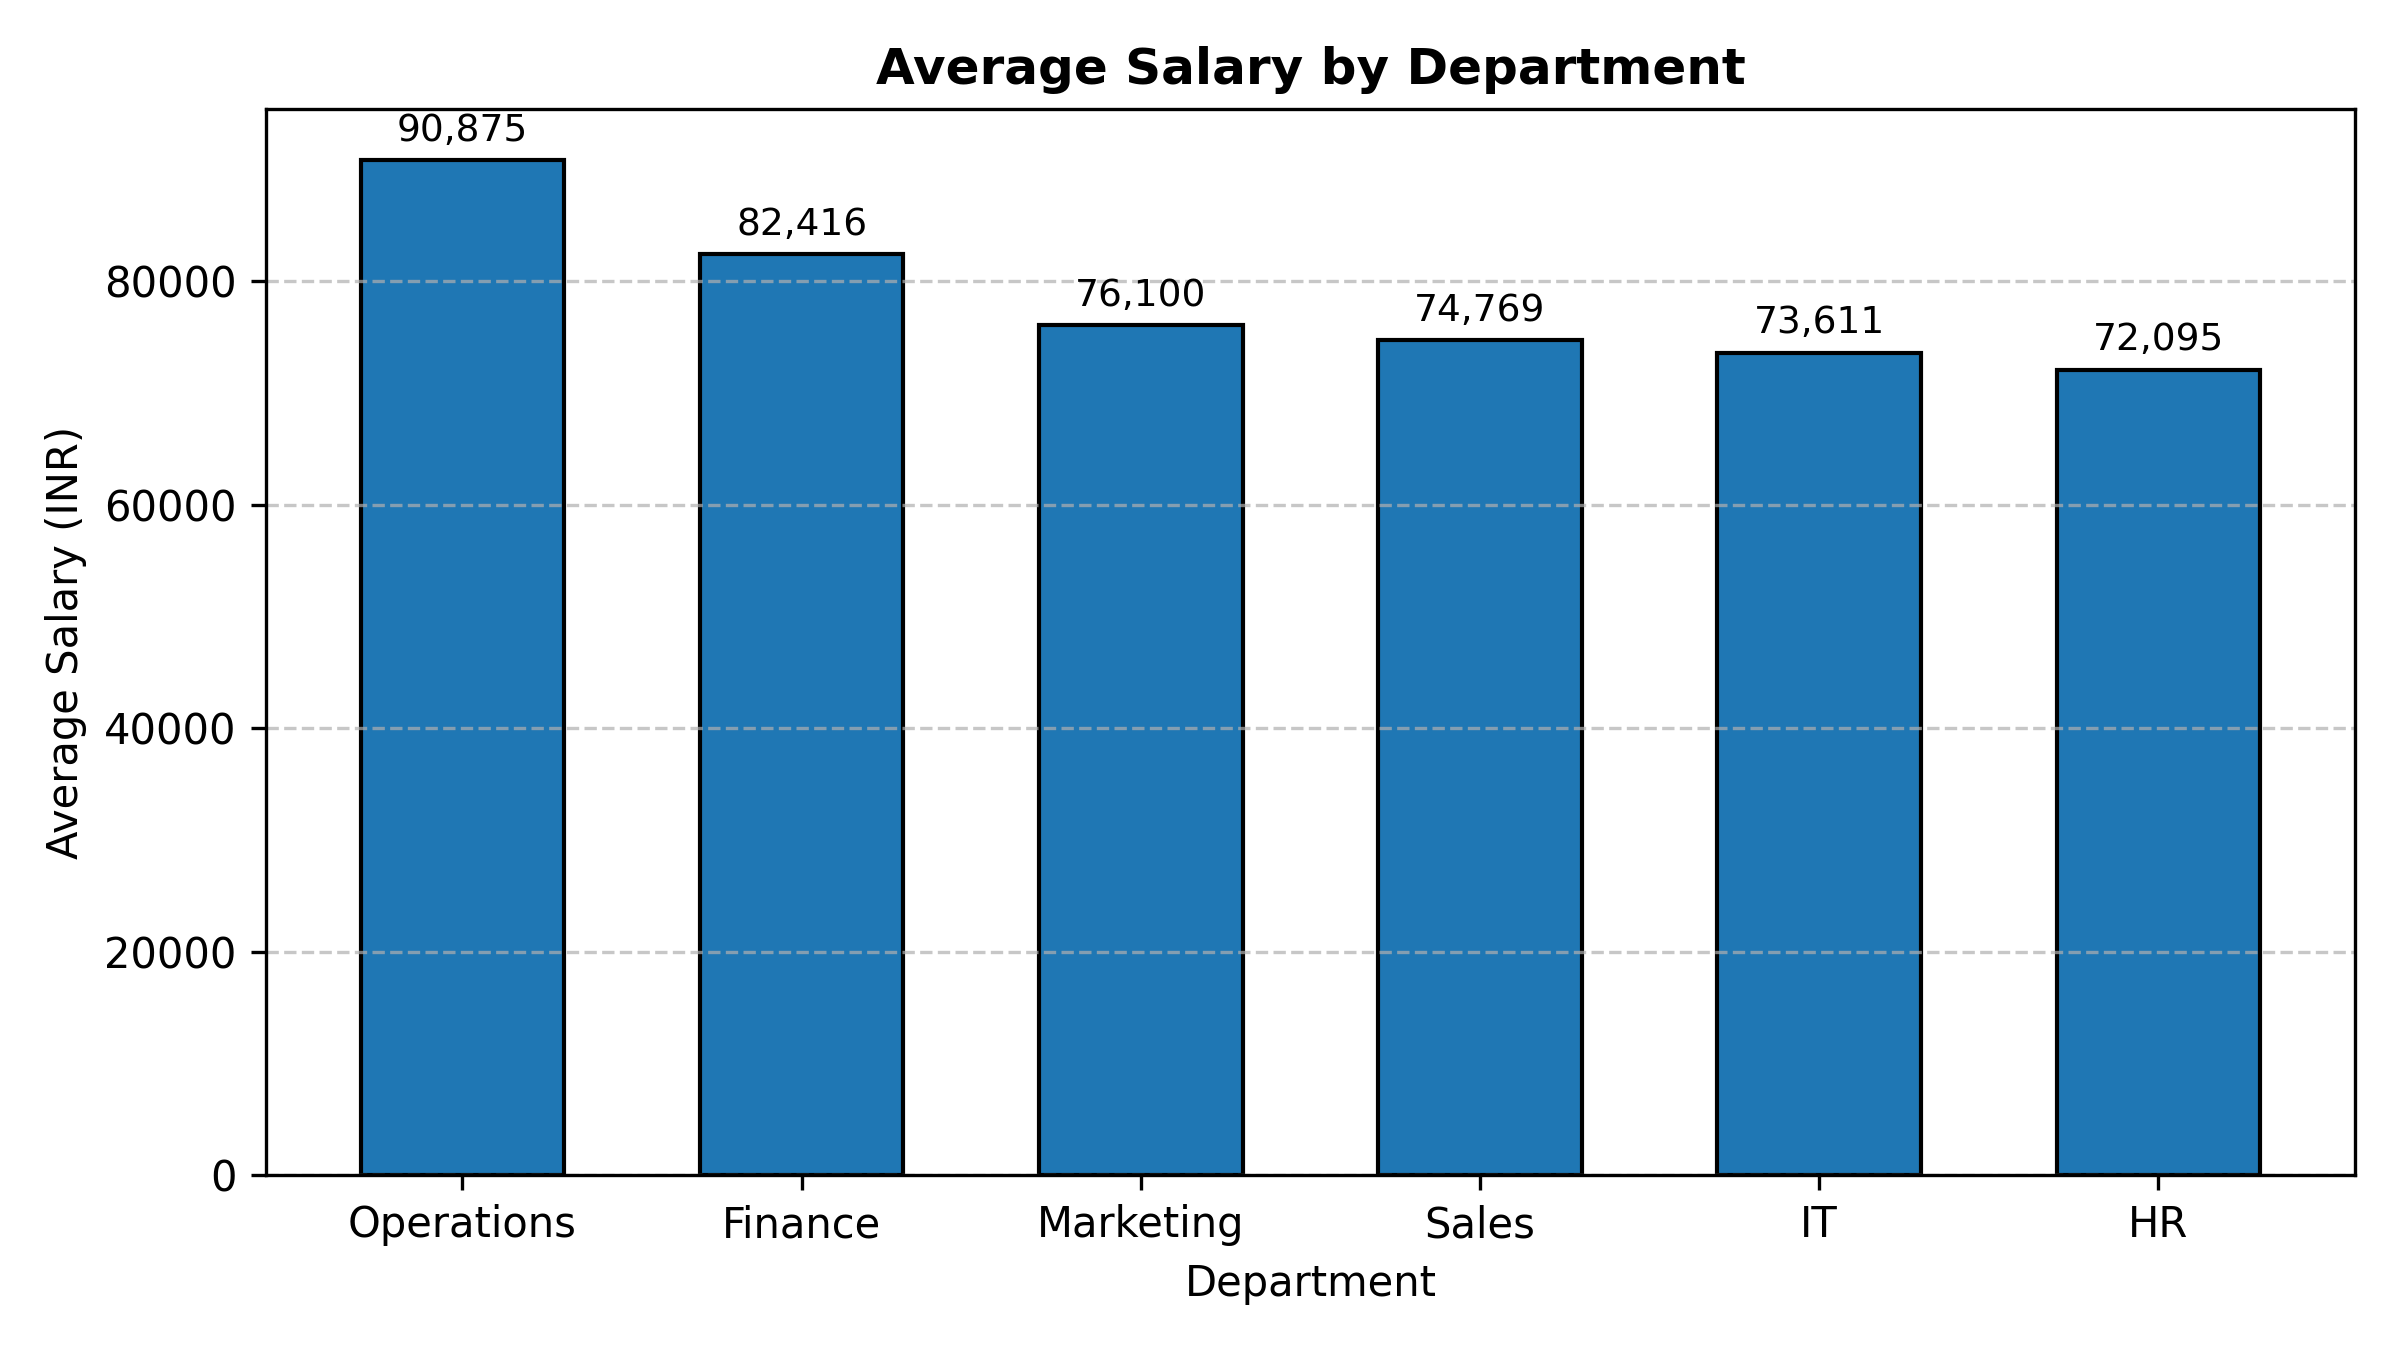
\includegraphics[width=\textwidth]{report_assets/exp1_avg_salary_dept.png}
        \caption{Average Salary by Department}
        \label{fig:exp1_salary_dept}
    \end{subfigure}
    \hfill
    \begin{subfigure}[b]{0.48\textwidth}
        \centering
        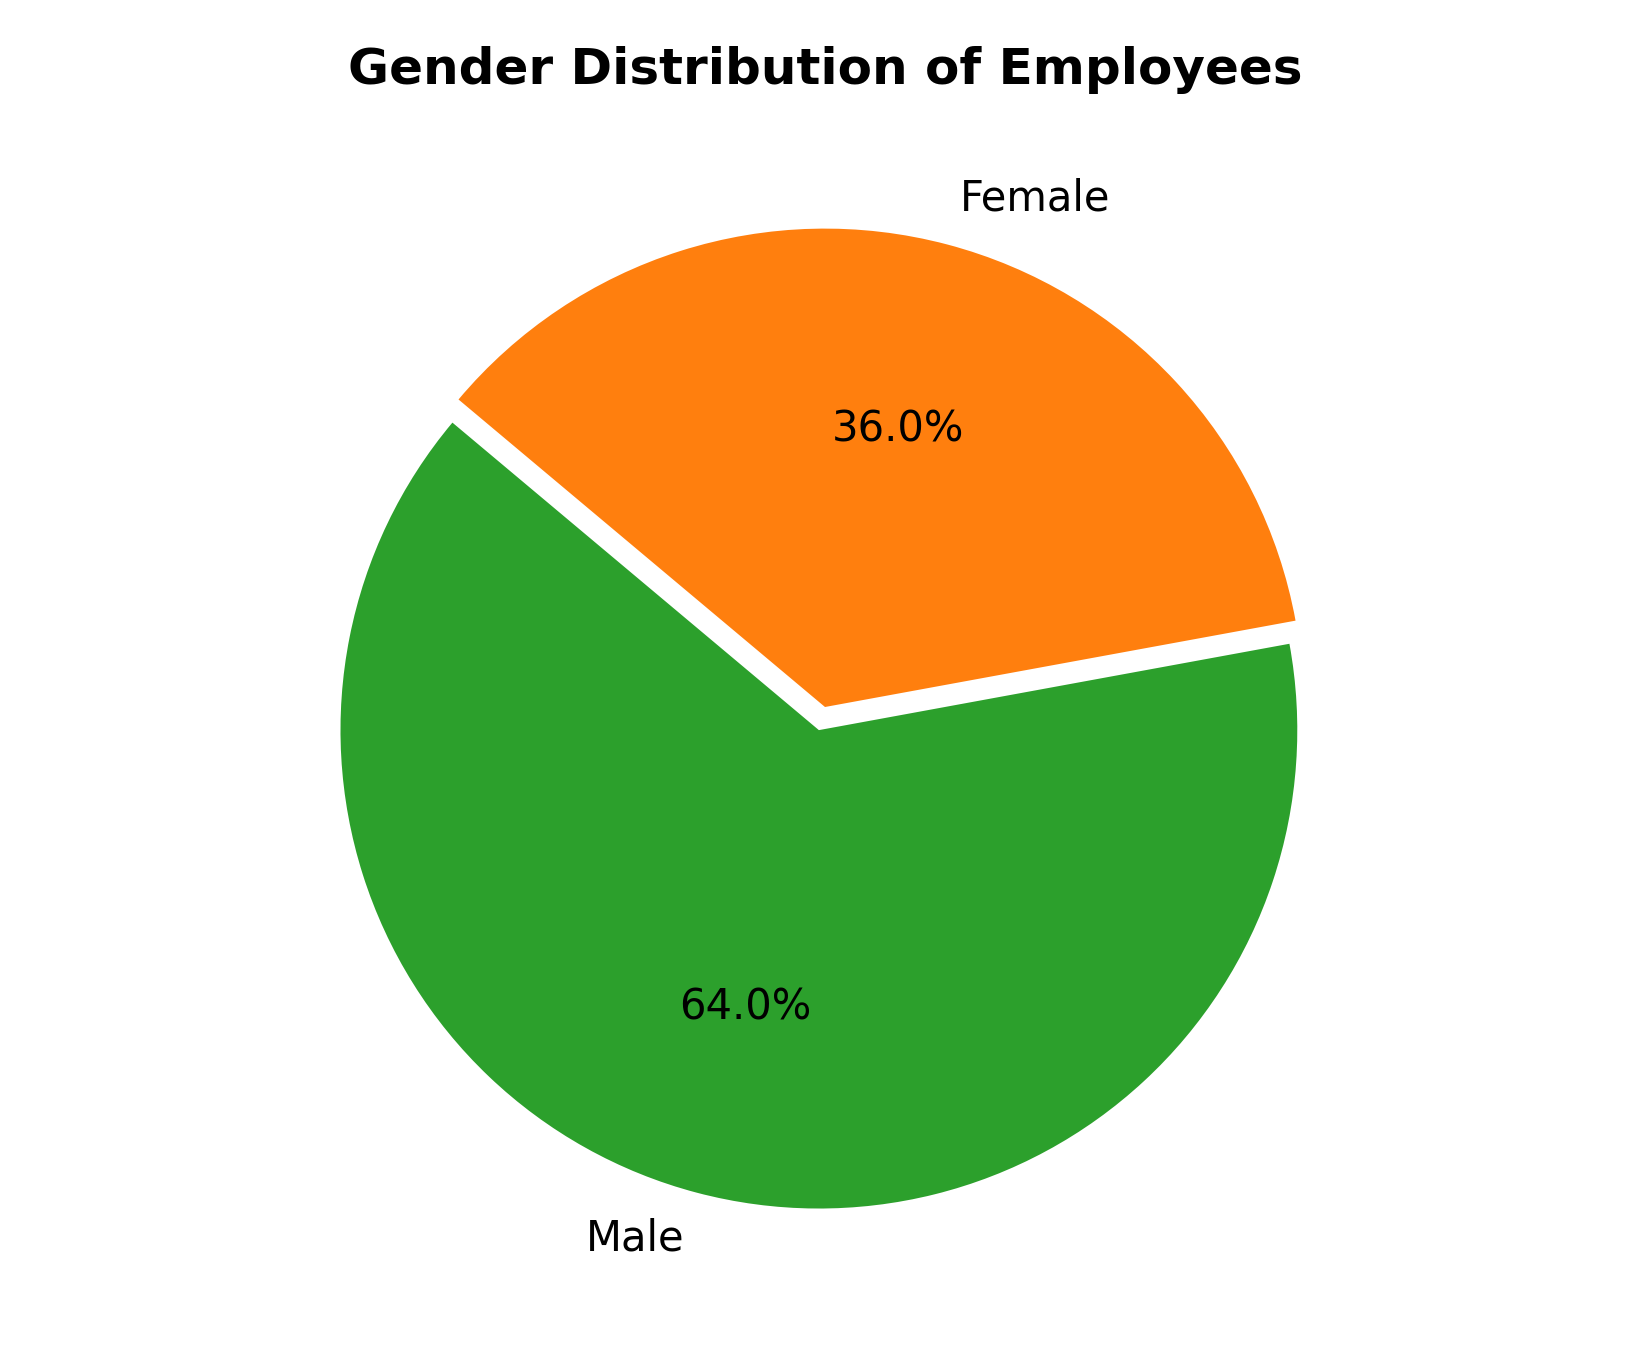
\includegraphics[width=\textwidth]{report_assets/exp1_gender_distribution.png}
        \caption{Gender Distribution Proportion}
        \label{fig:exp1_gender_pie}
    \end{subfigure}
    \vskip\baselineskip
    \begin{subfigure}[b]{0.48\textwidth}
        \centering
        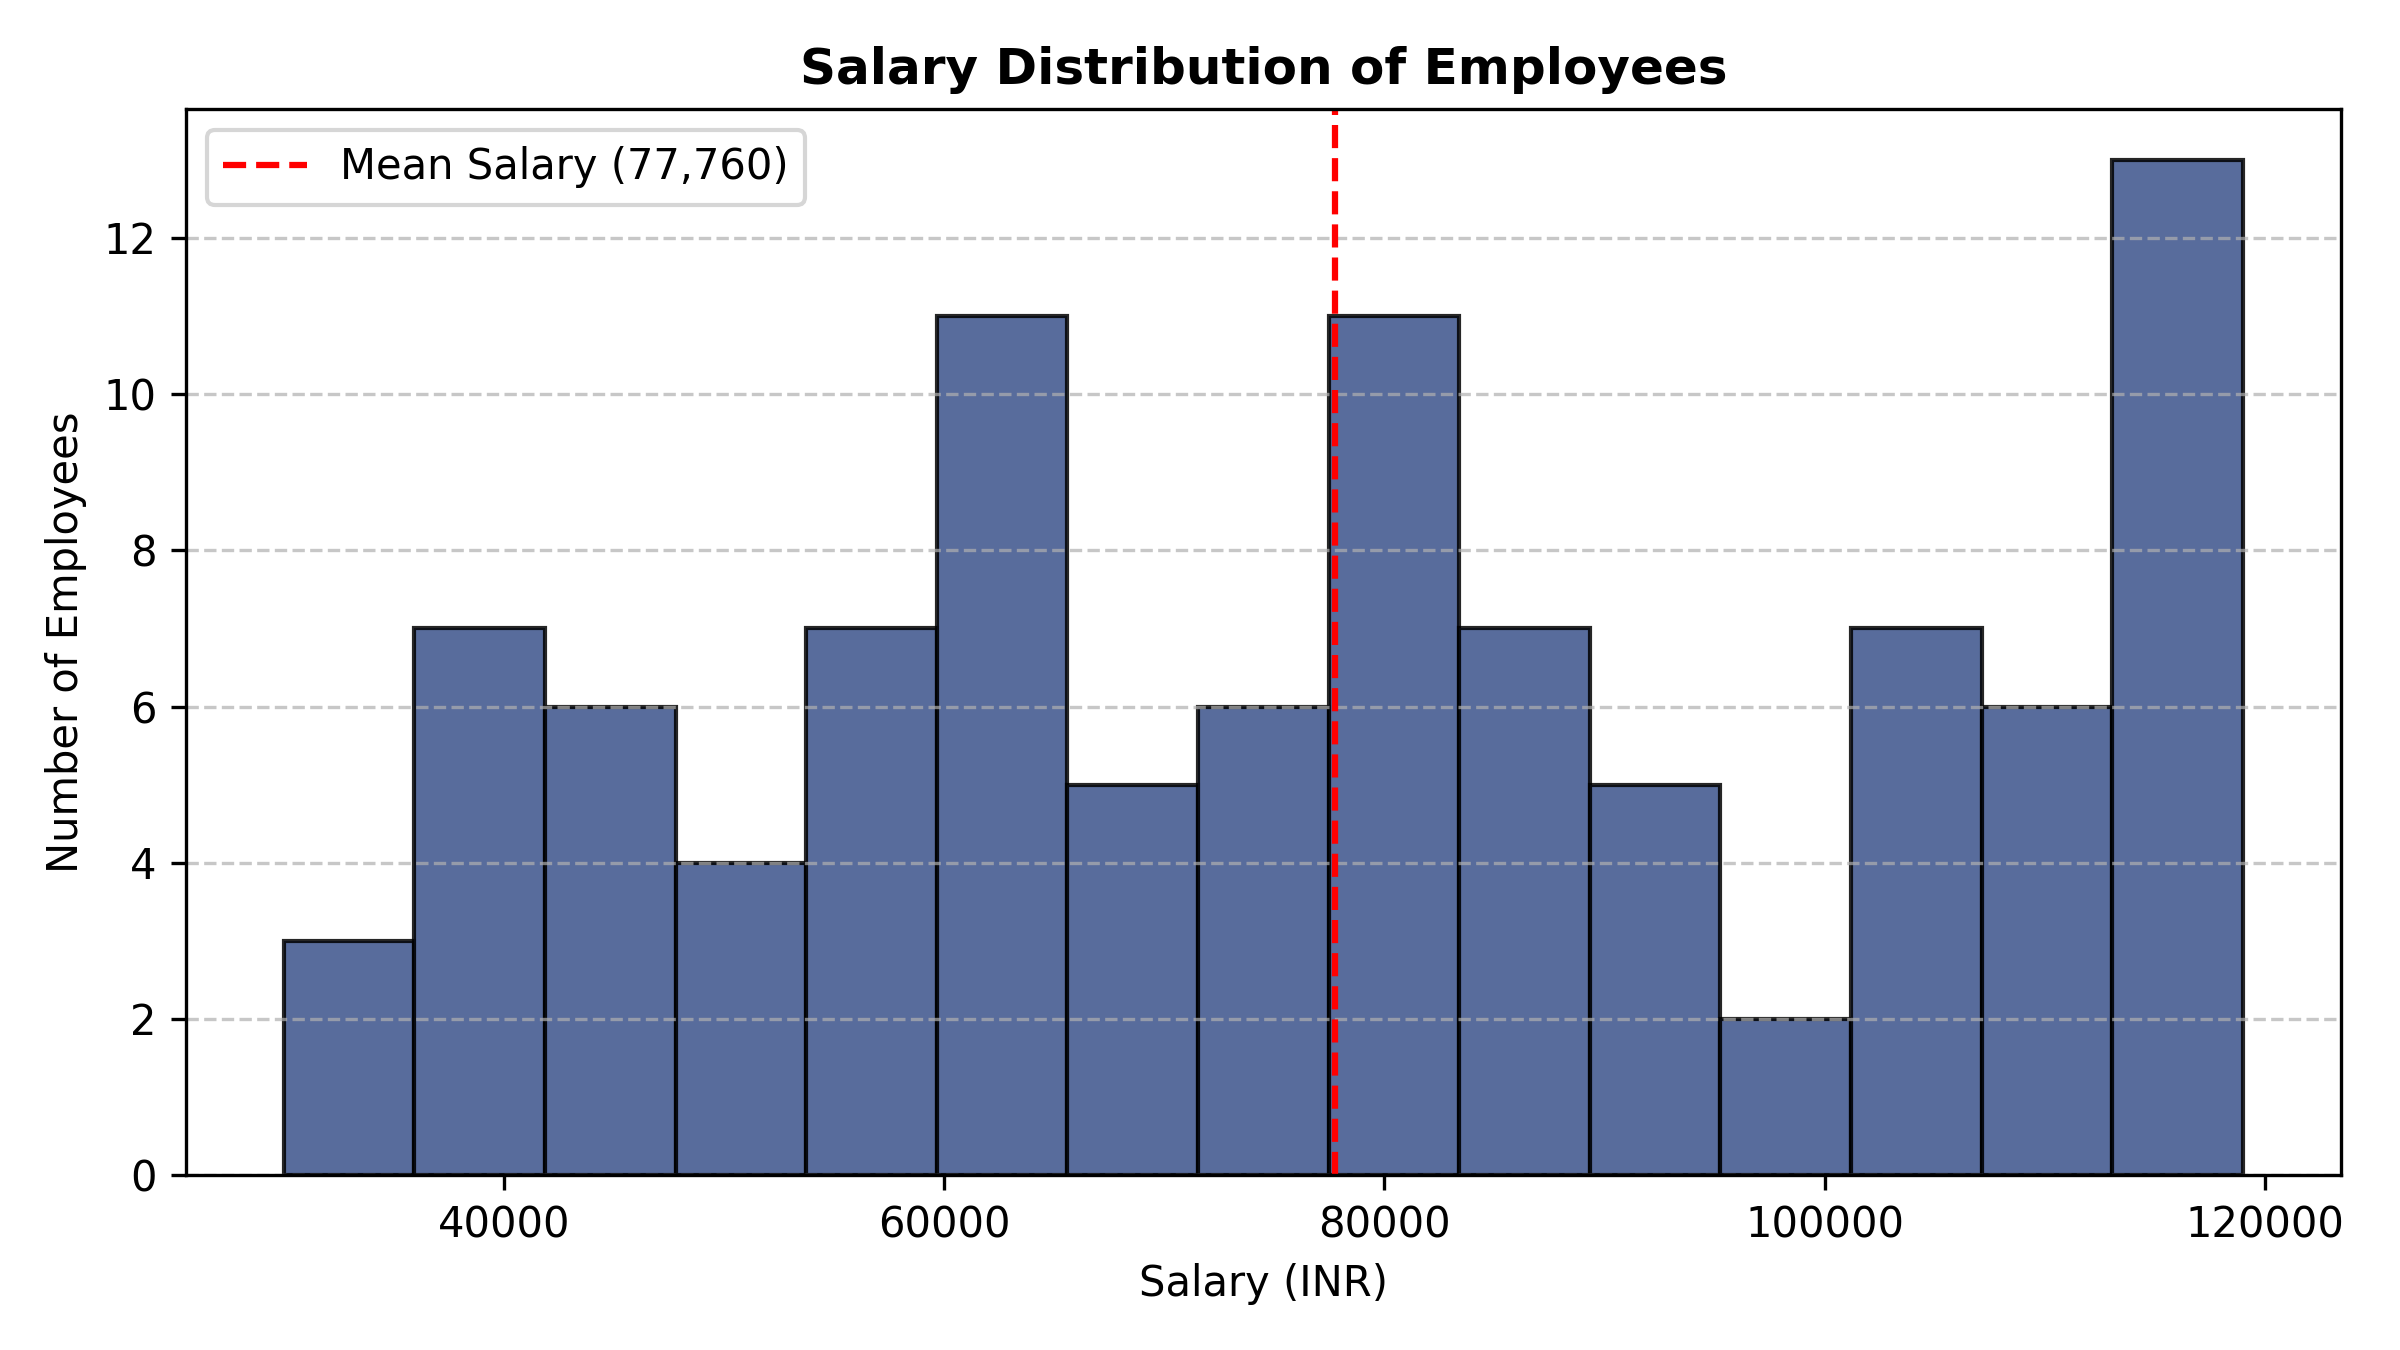
\includegraphics[width=\textwidth]{report_assets/exp1_salary_distribution.png}
        \caption{Salary Distribution Histogram}
        \label{fig:exp1_salary_hist}
    \end{subfigure}
    \hfill
    \begin{subfigure}[b]{0.48\textwidth}
        \centering
        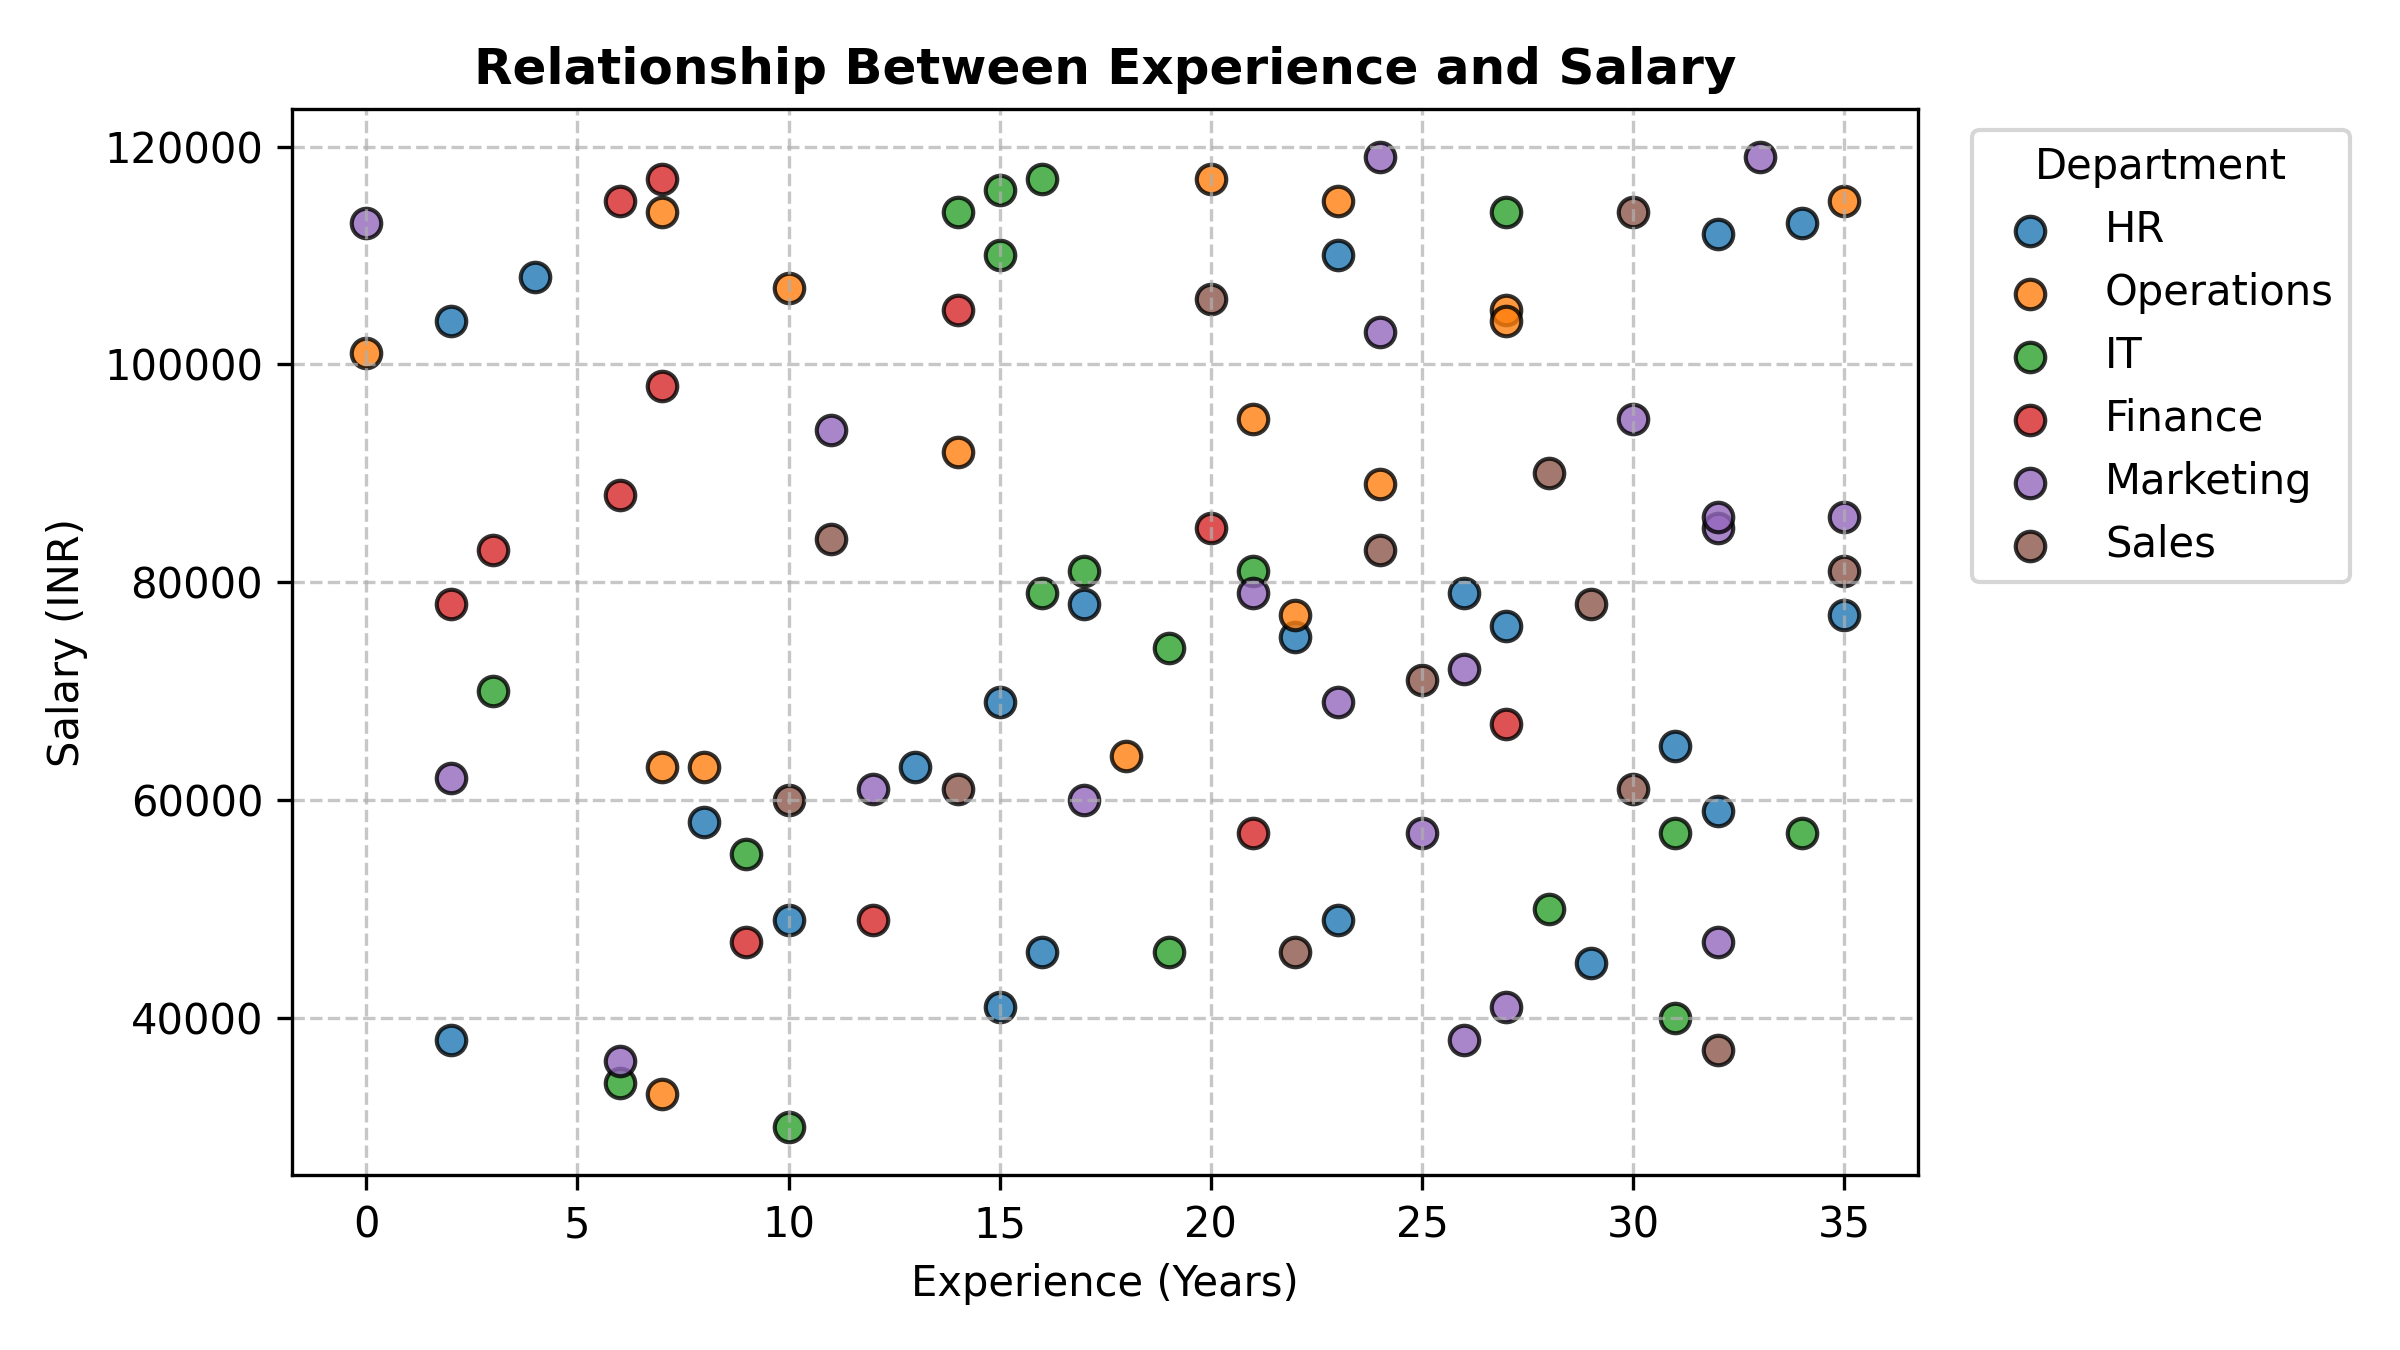
\includegraphics[width=\textwidth]{report_assets/exp1_experience_vs_salary.png}
        \caption{Experience vs. Salary by Department}
        \label{fig:exp1_exp_salary}
    \end{subfigure}
    \caption{Visual Exploratory Data Analysis Diagnostics for Experiment 1}
    \label{fig:exp1_all_plots}
\end{figure}

\begin{figure}[H]
    \centering
    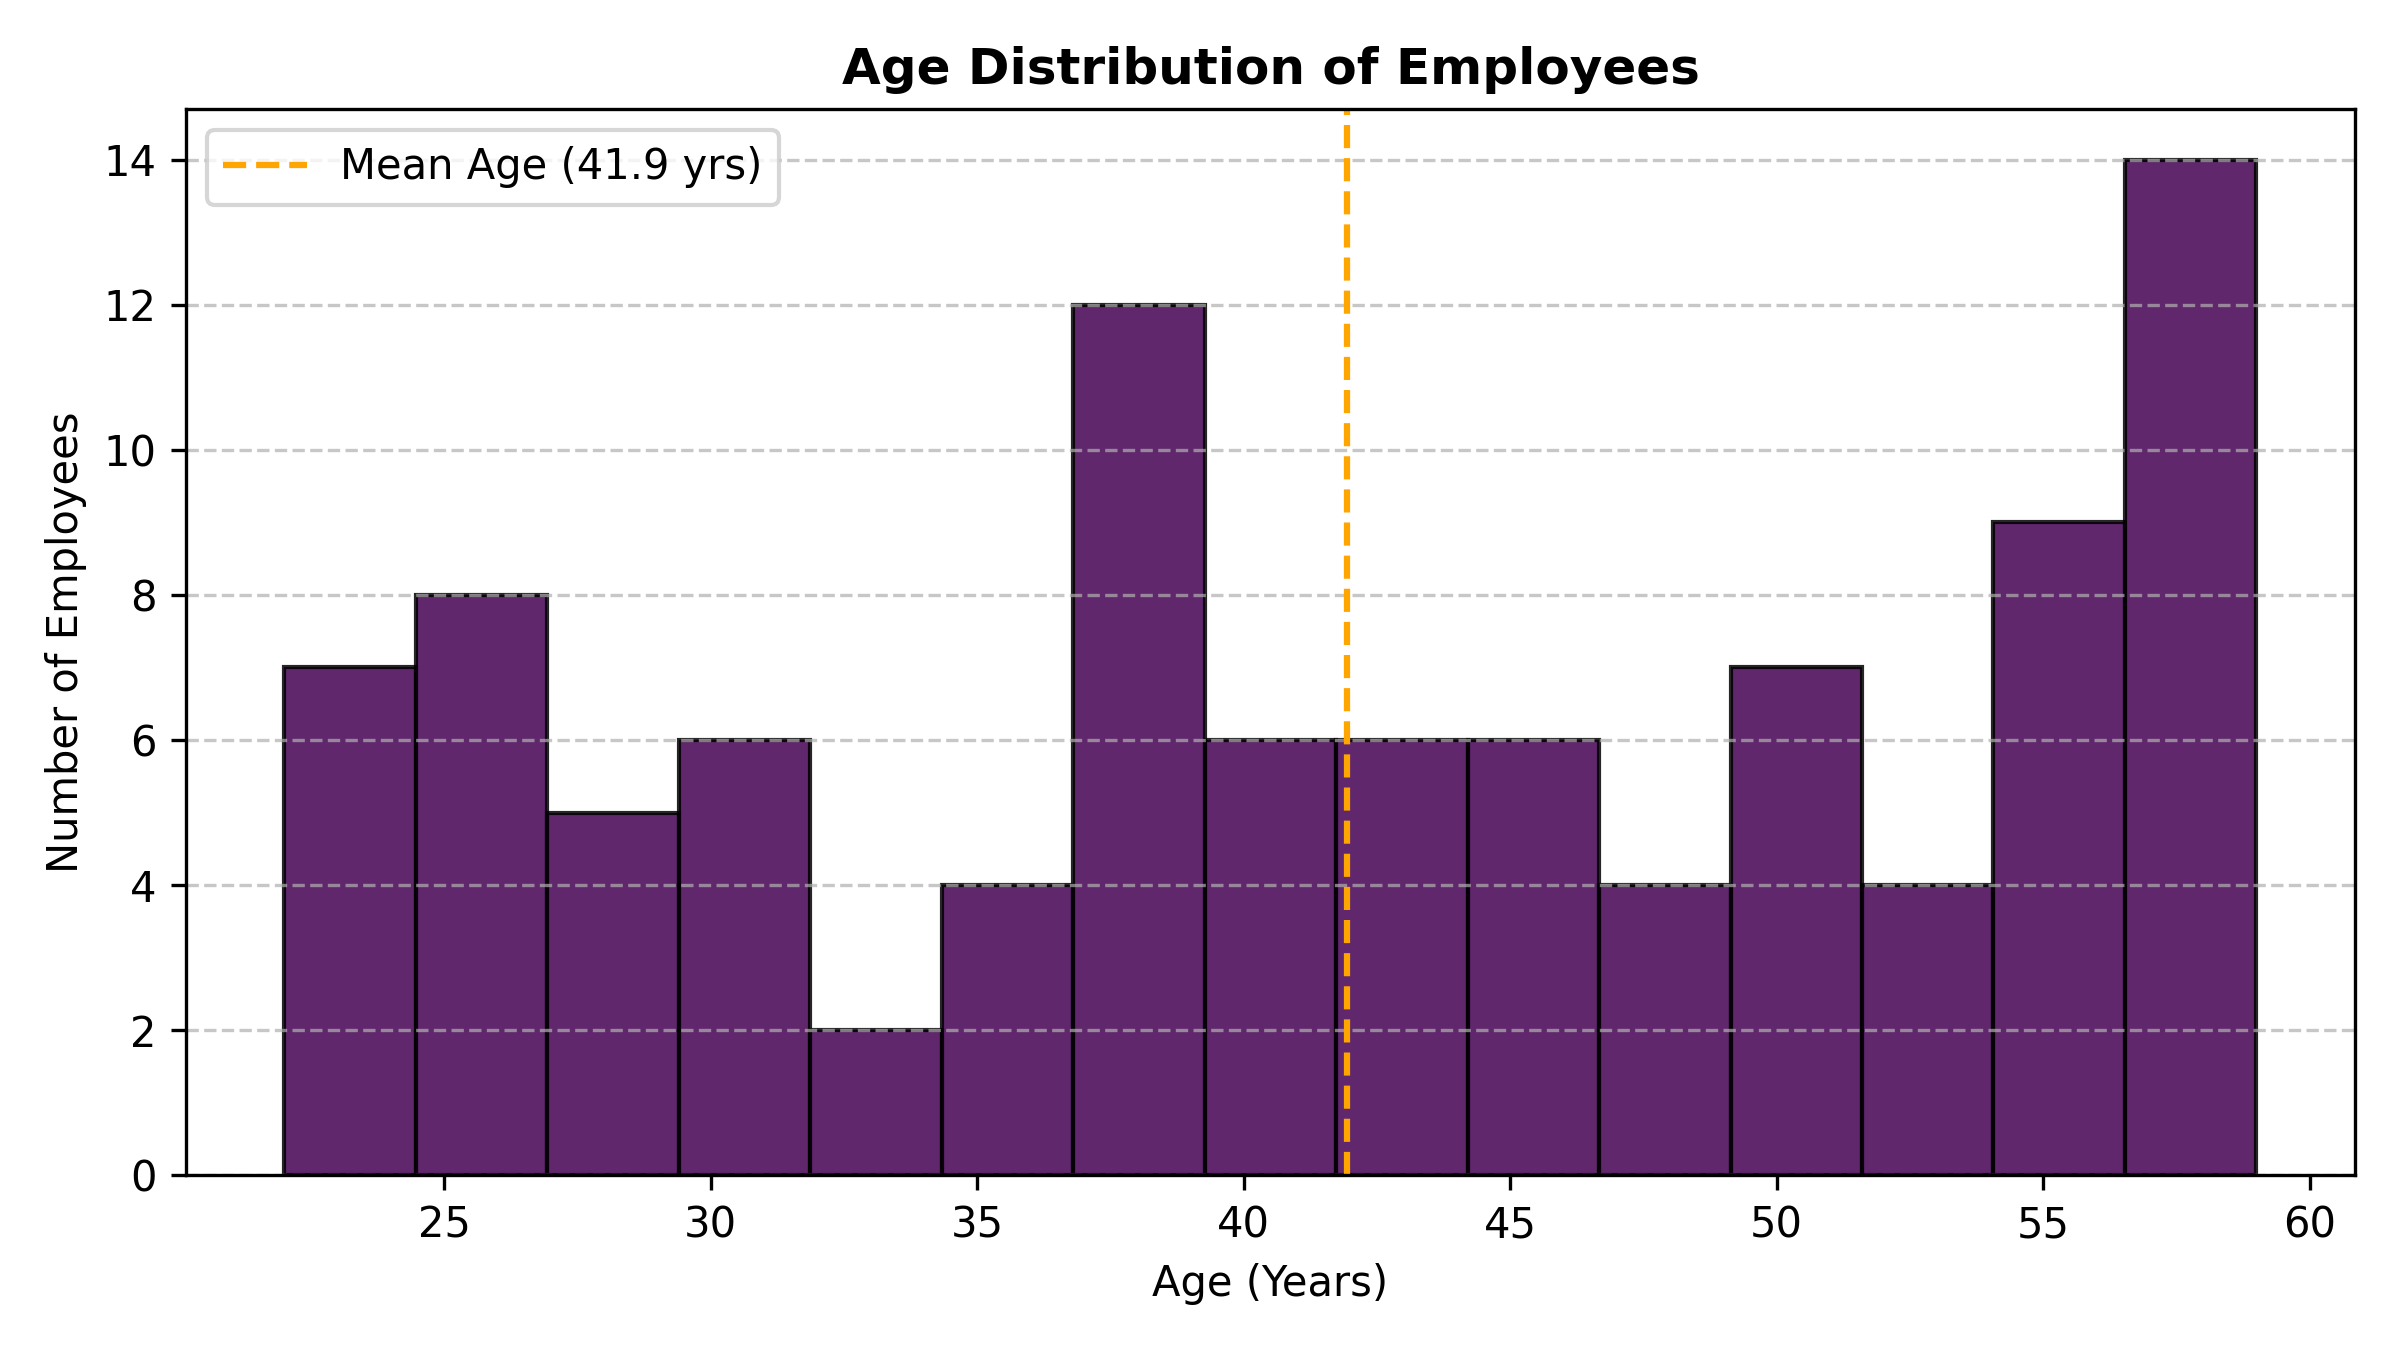
\includegraphics[width=0.65\textwidth]{report_assets/exp1_age_distribution.png}
    \caption{Employee Age Distribution Histogram across the Corporate Cohort}
    \label{fig:exp1_age_dist}
\end{figure}

\subsection{Top Corporate Earners and High-Remuneration Cohort}
Executing \texttt{df.nlargest(10, 'Salary')} isolates the top 10 highest-earning personnel as recorded in Table~\ref{tab:exp1_top10}.
\begin{table}[H]
\centering
\small
\caption{Top 10 Highest-Paid Employees in the Enterprise}
\label{tab:exp1_top10}
\begin{tabular}{llllrrr}
\toprule
\textbf{Emp. ID} & \textbf{Name} & \textbf{Department} & \textbf{Gender} & \textbf{Age} & \textbf{Salary (INR)} & \textbf{Experience} \\
\midrule
\texttt{E008} & Nisha8 & IT & Female & 58 & 119,000 & 28 \\
\texttt{E044} & Anjali44 & Marketing & Male & 46 & 118,000 & 21 \\
\texttt{E055} & Pooja55 & Sales & Female & 55 & 118,000 & 32 \\
\texttt{E076} & Bob76 & IT & Male & 56 & 118,000 & 34 \\
\texttt{E011} & Nisha11 & Finance & Male & 53 & 117,000 & 16 \\
\texttt{E085} & Bob85 & Marketing & Male & 57 & 117,000 & 28 \\
\texttt{E020} & Diana20 & Operations & Male & 45 & 114,000 & 15 \\
\texttt{E004} & Neha4 & HR & Male & 57 & 113,000 & 34 \\
\texttt{E071} & Neha71 & HR & Female & 56 & 113,000 & 29 \\
\texttt{E087} & Neha87 & IT & Male & 55 & 113,000 & 28 \\
\bottomrule
\end{tabular}
\end{table}

Furthermore, exactly 51 of the 100 employees ($51.0\%$) earn strictly above the corporate average salary of INR~77,760, indicating a balanced, non-skewed compensation distribution across the corporate hierarchy.

\section{Conclusion}
Experiment~1 successfully demonstrates the end-to-end execution of exploratory data analysis, statistical profiling, and categorical aggregation on tabular enterprise records. All ten curricular objectives were realized:
\begin{enumerate}
    \item Ingestion and validation verified a clean 100-record dataset with zero missingness across demographic and professional attributes.
    \item Departmental aggregations revealed that Finance commands the highest remuneration average ($\text{INR } 90,167$), while HR records the lowest average compensation ($\text{INR } 66,952$) despite hosting the largest headcount ($N = 21$).
    \item Demographic analysis identified a 64\% Male to 36\% Female distribution.
    \item The bivariate scatter plot between professional experience and compensation demonstrates positive overall correlation modulated by departmental compensation scaling.
\end{enumerate}
The exploratory profiling confirms that data understanding and descriptive sanitation provide an indispensable foundation for higher-order natural language processing pipelines and predictive modelling.
